\documentclass{beamer}
\usepackage{beamerthemeCambridgeUS}
\usepackage{color}  % for \textcolor{red}{blah}
\usepackage{graphicx}
\usepackage{subfigure}
\usepackage{multicol}
\usepackage{verbatim} % for \begin{comment}
\usepackage{lipsum}


\newcommand\Fontvi{\fontsize{6}{7.2}\selectfont}


\newenvironment{packed_enum}{
\begin{enumerate}
  \setlength{\itemsep}{1pt}
  \setlength{\parskip}{0pt}
  \setlength{\parsep}{0pt}
}{\end{enumerate}}

\newenvironment{packed_item}{
\begin{itemize}
  \setlength{\itemsep}{1pt}
  \setlength{\parskip}{0pt}
  \setlength{\parsep}{0pt}
}{\end{itemize}}

\usetheme{CambridgeUS}

\title{Discrete Mathematics}
\author[Geoffrey Buhl]{Geoffrey Buhl \\ \texttt{geoffrey.buhl@csuci.edu}}
\institute[CSUCI]{California State University Channel Islands}
\date{week 7 class 2}

\def \vec{{\rm vec}}
\newtheorem{conjecture}[theorem]{Conjecture}
\newtheorem{explanation}[theorem]{Explanation}


\begin{document}

%\frame{\titlepage}

%\section[Outline]{}
%\frame{\tableofcontents}

\section{Week 7 Class 2}


\frame
{
  \frametitle{Solving Non-homogenous Recurrence Relations}

Today we continue  develop a second method for solving non-homogenrous recurrence relations, using the auxiliary equation.

\vfill
Class Session Goals:
\begin{packed_enum}
\item Practice creating recurrence relations
\item Demonstrate elimination non-homogenous terms in recurrence
\end{packed_enum}
\vfill
}

\frame
{
  \frametitle{Some Non-homogenous Recurrences}

{\bf von Neuman Neighborhods} (A001844)\\ $V_n=V_{n-1}+4(n-1)$ with $V_0=1$\vfill
{\bf Tower of Hanoi} (A001787)\\$H_n=2H_{n-1}+1$ with $H_1=1$ \vfill
{\bf $2\times 2n$ binary matrices with $n+1$ 1s} (A000124)\\ $a_n=2a_{n-1}+2^{n-1}$ with $a_1=1$\vfill
{\bf Lazy Caterer} (A000124)\\ $c_n=c_{n-1}+n$ with $c_0=1$\vfill

}

\begin{comment}
\frame
{
  \frametitle{Important Taylor Series}


$\frac{1}{1-x}=1+x+x^2+x^3+x^4+x^5+x^6+ \cdots=\sum_{n=0}^{\infty}x^n$\vfill
$\frac{1}{(1-x)^2}=1+2x+3x^2+4x^3+5x^4+6x^5+ \cdots=\sum_{n=0}^{\infty}(n+1)x^n$\vfill
$\frac{1}{(1-x)^3}=1+3x+6x^2+10x^3+15x^4+21x^5+ \cdots=\sum_{n=0}^{\infty}\frac{(n+1)(n+2)}{2}x^n$\vfill
$\frac{x}{(1-x)^3}=1x+3x^2+6x^3+10x^4+15x^5+21x^6+ \cdots=\sum_{n=0}^{\infty}\frac{n(n+1)}{2}x^n$\vfill
$\frac{1}{1-\alpha x}=1+\alpha x+\alpha^2x^2+\alpha^3x^3+\alpha^4x^4+\alpha^5x^5+ \cdots=\sum_{n=0}^{\infty}\alpha^nx^n$\vfill
$\frac{1}{(1-\alpha x)^2}=1+2\alpha x+3\alpha^2x^2+4\alpha^3x^3+5\alpha^4x^4+6\alpha^5x^5+ \cdots=\sum_{n=0}^{\infty}(n+1)\alpha^nx^n$\vfill


}
\end{comment}

\frame
{
  \frametitle{Nested Triangular Numbers}
  
  Figurative numbers with shapes with 3 sides.

\begin{figure}[htp]
  \begin{center}
    \subfigure{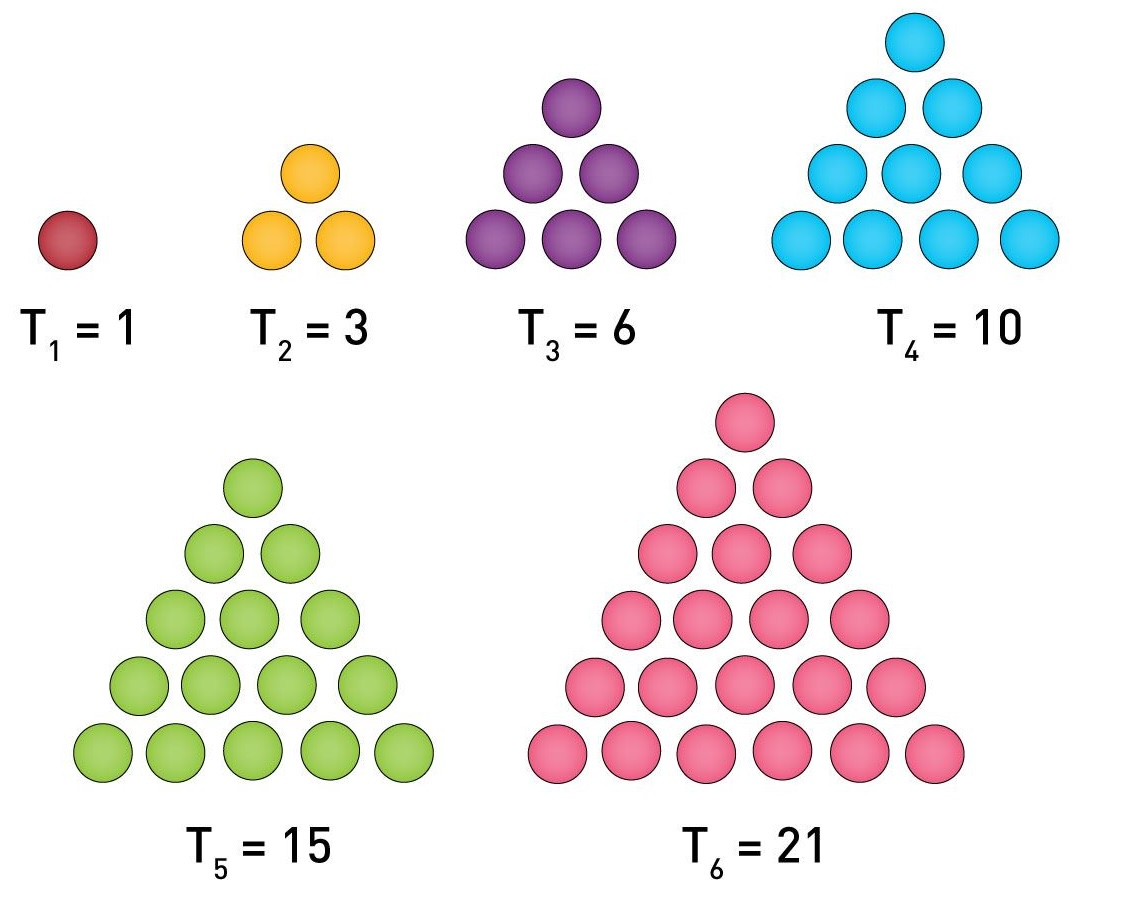
\includegraphics[scale=.15]{triangular-numbers.jpg}}
  \end{center}
\end{figure}

$T_n=T_{n-1}+n$ with $T_1=1$ (A000217). 
}




\frame
{
  \frametitle{Nested Square Numbers}
  
  Figurative numbers with shapes with 4 sides.

\begin{figure}[htp]
  \begin{center}
    \subfigure{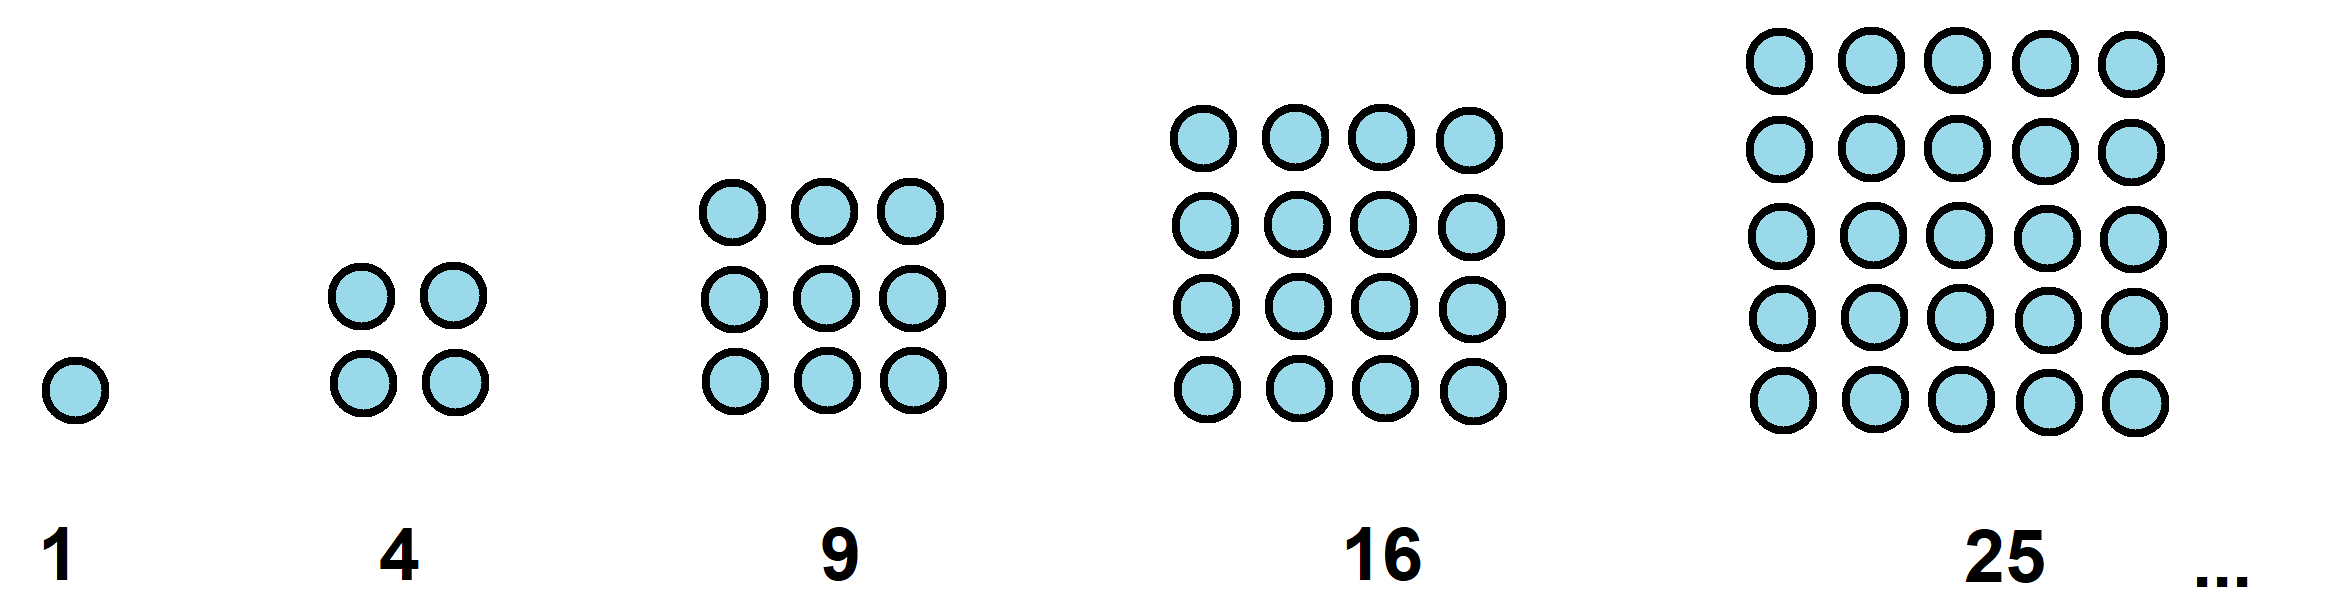
\includegraphics[scale=.12]{Fz_EG9VaEAATq-5.png}}
  \end{center}
\end{figure}

$S_n=S_{n-1}+2n-1$ with $S_1=1$ (A000290).

}


\frame
{
  \frametitle{Nested Pentagonal Numbers}

Figurative numbers with shapes with 5 sides.

\begin{figure}[htp]
  \begin{center}
    \subfigure{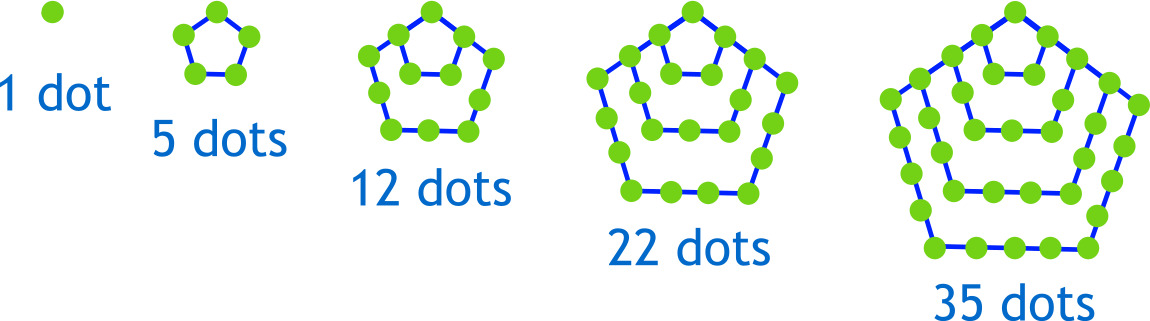
\includegraphics[scale=.25]{pentagonal-number-dots.jpg}}
  \end{center}
\end{figure}

$P_n=P_{n-1}+3n-2$ with $P_1=1$ (A000326).
}


\frame
{
  \frametitle{Calculation Demonstration}

\vfill
Exponential non-homogeneous terms with Towers of Hanoi recursion:
$H_n=H_{n-1}+2^{n-1}$ with $H_1=1$
\vfill
Polynomial non-homogeneous terms with Triangular numbers recursion:
$T_n=T_{n-1}+n$ with $T_1=1$
\vfill
}




\frame
{
  \frametitle{Now you try it}
Eliminate the non-homogenous term for the following recurrence relations:

{\bf Alternate Tower of Hanoi} (A001787)\\$H_n=2H_{n-1}+1$ with $H_1=1$ \vfill
{\bf $2\times 2n$ binary matrices with $n+1$ 1s} (A000124)\\ $a_n=2a_{n-1}+2^{n-1}$ with $a_1=1$\vfill
{\bf von Neuman Neighborhods} (A001844)\\ $V_n=V_{n-1}+4(n-1)$ with $V_0=1$\vfill
{\bf Square Numbers} (A000290)\\ $S_n=S_{n-1}+2n-1$ with $S_1=1$\vfill

}





\frame
{
  \frametitle{Nested Hexagonal Numbers}

\begin{figure}[htp]
  \begin{center}
    \subfigure{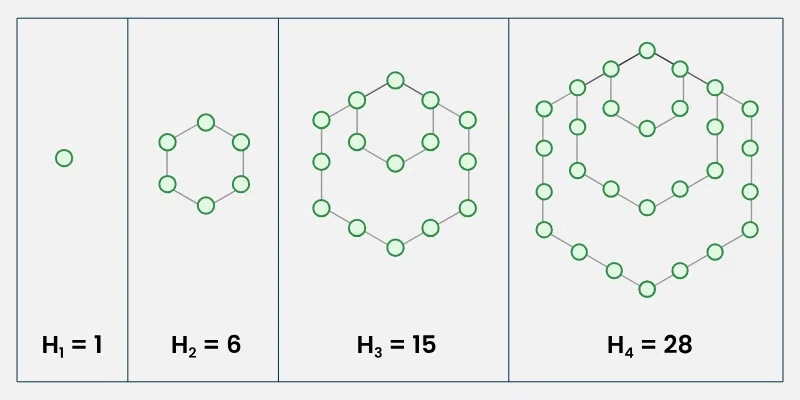
\includegraphics[scale=.25]{Hexagonal-Numbers.jpeg}}
  \end{center}
\end{figure}

Let $H_n$ be the number of dots in the $n$-th nested hexagon.
}


\frame
{
  \frametitle{Centered Triangular Numbers}

\begin{figure}[htp]
  \begin{center}
    \subfigure{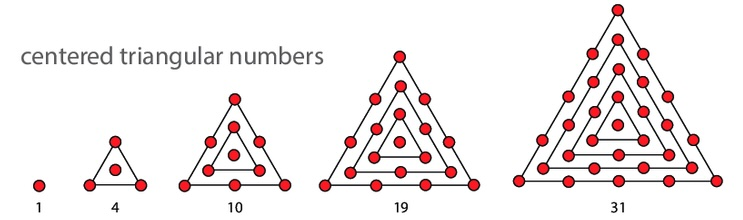
\includegraphics[scale=.4]{centered triangular}}
  \end{center}
\end{figure}

Let $\mathcal{T}_n$ be the be the number of dots in the $n$-th center nested triangle.  }




\frame
{
  \frametitle{Centered Square Numbers}

\begin{figure}[htp]
  \begin{center}
    \subfigure{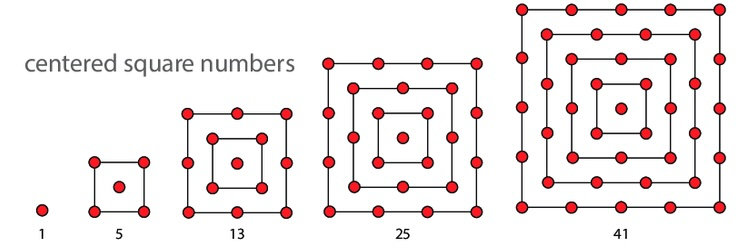
\includegraphics[scale=.4]{centered square}}
  \end{center}
\end{figure}

Let $\mathcal{S}_n$ is the number of  dots in the $n$-th center nested square .  }

\frame
{
  \frametitle{Centered Pentagonal Numbers}

\begin{figure}[htp]
  \begin{center}
    \subfigure{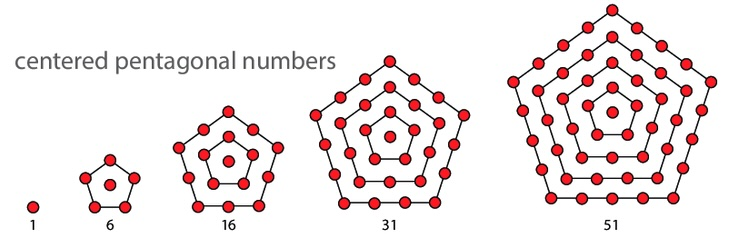
\includegraphics[scale=.4]{centered pentagonal}}
  \end{center}
\end{figure}

Let $\mathcal{P}_n$ be the number of dots in the $n$-th center nested pentagon.  Can you express $\mathcal{P}_n$ as a recurrence relation?  What's it's generating function?  Can you find a closed form solution? }


\frame
{
  \frametitle{Centered Hexagonal Numbers}

\begin{figure}[htp]
  \begin{center}
    \subfigure{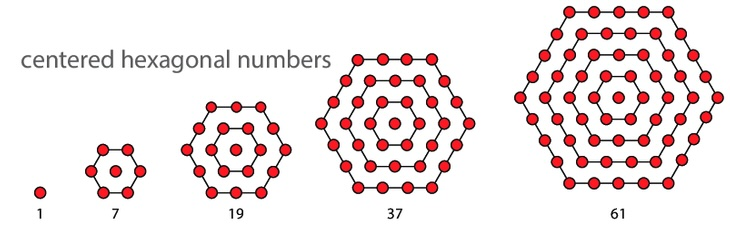
\includegraphics[scale=.4]{centered hexagonal}}
  \end{center}
\end{figure}

Let $\mathcal{H}_n$ be the number of dots in the $n$-th center nested hexagon.  Can you express $\mathcal{H}_n$ as a recurrence relation?   What's it's generating function?  Can you find a closed form solution?}

\frame
{
  \frametitle{Activity}

$H_n=(1,6,15,28, 45, \ldots)$\\
$\mathcal{T}_n=(1,4,10,19,31, \ldots)$\\
$\mathcal{S}_n=(1,5,13,25,41, \ldots)$\\
$\mathcal{P}_n=(1,6,16,31,51, \ldots)$\\
$\mathcal{H}_n=(1,7,19,37,61, \ldots)$\\
\vfill

Choose one of these new figurative numbers and answer the following questions:  What is the recurrence relationship?  What is the recurrence relationship if you convert it into a homogeneous recurrence? What is the close form solution?

\vfill
}



\begin{comment}
\frame
{
  \frametitle{Frogs and Toads Puzzle}

 Below is the $n=3$ version of the puzzle.
\begin{figure}[htp]
  \begin{center}
    \subfigure{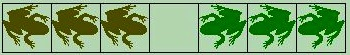
\includegraphics[scale=.4]{frogs}}
  \end{center}
\end{figure}

Let $m_n$ be the minimum number of moves (jumps or slides) in a winning strategy.  Can you express $m_n$ as a recurrence relation?  What's it's generating function?  Can you find a closed form solution?
%(A005563)
%a(n) = a(n-1) + 2*n + 1 


}



\frame
{
  \frametitle{Creating Recursion Activity}

In small groups, work on the ``Pancakes and Ternary Strings'' worksheet. The goals of this worksheet are to:
\vfill
\begin{packed_enum}
\item Practice finding a non-homogeneous generating function of a sequence.
\end{packed_enum}
\pause
\vfill
\underline{Problem 1 answer}\\ $c_n=c_{n-1}+n$ with $c_0=1$ (A000124)
\pause
\vfill
\underline{Problem 2 answer}\\ $x_n=x_{n-1}+x_{n-2}+2^{n-2}$ with $x_0=0$ and $x_1=0$ (A008466)

}

\frame
{
  \frametitle{Eliminate a polynomial non-homogeneous term}
{\bf Lazy Caterer Problem}
Solve $c_n=c_{n-1}+n$ with $c_0=1$ using the auxiliary equation method. \vfill

Subtract $c_{n-1}=c_{n-2}+(n-1)$ and .... \vfill
\pause
Answer 	
$c_n =\frac{n^2}{2}+\frac{n}{2}+1$
}

\frame
{
  \frametitle{Eliminate an exponential non-homogeneous term}

Solve $x_n=x_{n-1}+x_{n-2}+2^{n-2}$ with $x_0=0$ and $x_1=0$  using the auxiliary equation method. \vfill

Subtract $2(x_{n-1}=x_{n-2}+x_{n-3}+2^{n-3})$.\vfill

\pause
Answer
$$x_n=\frac{2 \sqrt{5} \left(\frac{\sqrt{5}}{2}+\frac{1}{2}\right)^n-(15-5 \sqrt{5}) 2^n+(15-7 \sqrt{5}) \left(\frac{1}{2}-\frac{\sqrt{5}}{2}\right)^n}{5 \left(\sqrt{5}-3\right)}$$
}
\end{comment}

\end{document}

